\documentclass[12pt,a4paper,pdftex]{article}

% Sprache
\usepackage[ngerman]{babel}

\usepackage[utf8]{inputenc}

\usepackage{graphicx}

% Page layout
\usepackage{geometry}
\geometry{a4paper,lmargin={2.5cm}, rmargin={2.5cm}, tmargin={2cm}, bmargin={2.5cm}}

% Figure and Caption layout
\usepackage[bf]{caption}
\usepackage{subcaption}
\usepackage{wrapfig}

% Befehle zur Textauszeichnung (hervorheben, unterstreichen ect.)
\usepackage{color,soul}

% Zitier-Style für Bücher und URL
\usepackage[numbers]{natbib}
\usepackage[breaklinks=true,bookmarks=true,bookmarksopen=true,colorlinks=true,citecolor=black,linkcolor=black,urlcolor=gray,pdfpagemode=UseNone,pdfstartview=FitH]{hyperref}


\usepackage{float}
\usepackage{gensymb}
\usepackage{siunitx}
\usepackage{tabularx}
\usepackage{amsmath}

% for commenting a whole section
\usepackage{verbatim}

\usepackage{pgfgantt}
\usepackage{afterpage}

% Index
\usepackage{imakeidx}
\makeindex[intoc, columnseprule]
\newcommand{\indextitle}{\section{Index}}

% Bilder importieren
\usepackage{epstopdf}
\epstopdfDeclareGraphicsRule{.pdf}{png}{.png}{convert #1 \OutputFile}
\DeclareGraphicsExtensions{.png,.pdf}

% Bildernummerierung fuer jedes kapitel
\usepackage{chngcntr}
\counterwithin{figure}{section}

% ich hab keine ahnung was die tun und wir brauchen sie auch nicht
%\newcommand{\command}[1]{\texttt{#1}}
%\newcommand{\fileextension}[1]{\texttt{#1}}

% plus minus zeichen
\newcommand{\rpm}{\raisebox{.2ex}{$\scriptstyle\pm$} }

% kapitel title auf deutsch
\renewcommand{\bibsection}{\section{Literaturverzeichnis}}



%%%%%%%%%%%%%%%%%%%%%%%%%%%%%%%%%%%%%%%%%%%%%%%%%%%%%%%%%%%%%

\begin{document}
\setlength{\parindent}{0pt}

%%%%%%%%%%%%%%%%%%%%%%%%%%%%%%%%%%%%%%%%%%%%%%%%%%%%%%%%%%%%%
% Titelseite

\begin{titlepage}
 \begin{center}
        \vspace*{1cm}
        \LARGE
        \textbf{Kurzes Lehrbuch der Neuroanatomie des Säugers}
        \vspace{2cm}
        
        \Large
        Praktikumsprotokoll des Mastermoduls Neuroanatomie
        \vspace{4cm}
        
        \large
        vorgelegt von \\ Jacqueline Göbl, Julia Grüb, Marta Provenzano und Laura Seidler % Author name
        \vfill
        \large     
        T\"ubingen, \today
    \end{center}
    \newpage
        \thispagestyle{empty}
        \mbox{}
        \newpage
\end{titlepage}


\thispagestyle{empty}
\mbox{}
%%%%%%%%%%%%%%%%%%%%%%%%%%%%%%%%%%%%%%%%%%%%%%%%%%%%%%%%%%%%%% Inhaltsverzeichnis und Abbildungsverzeichnis

\tableofcontents
\newpage
\listoffigures

%%%%%%%%%%%%%%%%%%%%%%%%%%%%%%%%%%%%%%%%%%%%%%%%%%%%%%%%%%%%%
% Textbeginn

\newpage
\section{Einleitung}

\newpage
\section{Material und Methoden}

Computerprogramm am Aufnahmecomputer der Bilder:
Axio Vision (AxioVs40 4.8.2.0, Copyright 2006-2010, Carl zeiss MicroImaging GmBH)



\begin{itemize}
    \item Schafhirn - die Präperationsanleitungen hat auch Jacqui
    \item Perfusion der Ratte - hat auch Jacqui
    \item Färbungen (Nissl, Faser, Immunohistochemie)
    \item Auswertung am Mikroskop - Jacqui hat die genauen Angaben des Programms welches wir für die Mikroskopaufnahmen benutzt wurde
\end{itemize}

\newpage
\section{Allgemeine Übersicht}
\textcolor{red}{Hallo, ich schreibe in nem anderen Dokument und füge meine Sachen später ein: \\
\noindent https://www.overleaf.com/read/tcmxbnddrqvr}

\subsection{Äußere Morphologie und Hirnteile}
\subsection{Spezifische Lage der Hirnnervenkerne im Hirnstamm}
\begin{itemize}
    \item relative Lage in Bezug zu sensorischen und motorischen Funktionen; Bezug zur dorsoventralen Organisation des Rückenmarks  
    (motorische Kerne liegen systematisch wo anders als somatosensorische Kerne ---wegen der Auflösung der dorsoventralen Struktur zu einer medialen lateralen Struktur) 
    \item sensorisch: N.trigeminus, N.cochlearis, N.vestibularis, NTS
    \item motorisch: Mo5, Mo7, N. ocolomotorius
\end{itemize}

% Allgemeine sensorische Bahnen
\newpage
\section{Allgemeine sensorische Bahnen}
Dieses Kapitel behandelt die allgemeine Sensorik \index{Sensorik !allgemein} die im Gegensatz zu speziellen Sensorik (Kapitel~ \ref{sec:spezsens}) steht. In der allgemeine Sensorik sind die Sinne zusammen gefasst welche über den ganzen Körper verteilt sind, dazu gehören unter anderem die Somatosensorik \index{Sensorik !Somato-} die Propriozeption \index{Propriozeption} und die Viszerosensorik \index{Sensorik !Viszero-}\textsuperscript{\cite[22]{kandel2013principles}}. Die spezielle Sensorik \index{Sensorik !speziell} fasst die Sinne zusammen welche auf Grund der Cephalisation bei Säugern nach vorne in den Kopf verlagert sind.
\\
\noindent
Die Somatosensorik zeichnet sich durch die Repräsentation der direkten äußeren Welt und der inneren Welt aus. Bei der Repräsentation der Außenwelt unterscheidet man bei Säugetieren zwischen zwei Rezeptorsystemen. Zum einen die haarlose Haut in den Handinnenflächen, an der Fußunterseite und an den Lippen und der Nase, zum anderen die behaarte Haut mit hoch spezialisierten Tastsinneszellen innerviert durch die Bewegungen des Follikels auf den Blutsinus \index{Blutsinus} der Vibrissen.  \index{Sinushaar} \textsuperscript{\cite[24]{paxinos2014rat}}
Die Propriozeption codiert die Informationen der relative Position unserer Extremitäten und anderer Körperteile im Raum und bildet in den Vorderextremitäten die Grundlage für abstrakte Wahrnehmung von Objektgrößen und Gewicht. Ein weiteren Bereich in der Somatosensorik bildet der Sinn welcher Schmerzen und Temperatur verarbeitet. \textsuperscript{\cite[24]{paxinos2014rat}}
Im Weiteren wird am Beispiel der Ratte näher auf die unterschiedlichen Systeme eingegangen und wodurch diese sich genau unterscheiden. 


% Somatosensorik
\subsection{Somatosensorik \index{Somatosensorik} des Körpers}
Die Somatosensorik des Körpers wird in zwei Systeme unterteilt, wobei der Tastsinn \index{Tastsinn} und die Propriozeption das lemniskale System \index{System !lemniskal} bilden und der Schmerz- und Temperatursinn  das anterolaterales System. \index{System !anterolateral} Beide Systeme werden durch die Rezeptoren unter der haarlosen Haut der Säuger innerviert.

\subsubsection{Tastsinn und Propriozeption (lemniskales System)}

\subsubsection*{Rezeptoren}
Die Rezeptoren des lemniskalen Systems werden unterteilt, in ihre Lage unter der Haut und ihre Adaptationseigenschaften. Dadurch unterscheiden sie sich in der Modalität, die sie codieren. Bei der Lage wird unterschieden zwischen direkt unter der Oberfläche oder tiefer im Gewebe liegenden Nervenendigungen und schnell bzw. phasisch und langsam bzw. phasisch-tonisch Adaptation dieser Nerven.\\
Direkt unter der Hautoberfläche liegen die Meissner- und die Merkel-Rezeptoren welche für Bewegung und Druck sowie in abstrakterem Sinne für Form, Textur und das Greifen nach Objekten codieren. \textsuperscript{\cite[24]{paxinos2014rat}} Tiefer unter der Haut liegen die Pacini-Rezeptoren welche schnell adaptierende Rezeptoren sind, die für Vibrationen codieren. Zusammen mit den Meissner- und Merkelrezeptoren bilden sie den bewussten Tastsinn. Die Neurone der Rezeptoren sind dicke, myelinisierte A$\alpha$ Nervenfasern mit einer Leitgeschwindigkeit von 72-120 m/s \textsuperscript{\cite[22]{kandel2013principles}}. Unbewusst werden von den langsamen, tief unter der Haut liegenden Ruffini-Rezeptoren Informationen über die Dehnung der Haut und der Muskeln, damit der Position der Gelenke und Extremitäten weiter gegeben.
Die Nervenfasern der Propriozeption sind dicke, myelinisierte A$\beta$ Nerven deren Durchmesser etwas geringer ist als, der der A$\alpha$ Neuronen.
Die Nervenfasern eines Hautgebiets werden zu einem peripheren Nervenstrang gebündelt und ziehen in das Spinalganglion innerhalb des Wirbelkanals. Die Zellkörper der Nervenfasern liegen in diesem Spinalganglion und sind umgeben von speziellen Gliazellen. Zwischen den Nervenzellen verlaufen fenstrierte Kapillaren und versorgen die Nervenfasern mit den nötigen Nährstoffen. 

\subsubsection*{Rückenmark}
Die Axone der Nerven ziehen weiter in die Wirbelsäule. Da hier keine synaptische Verschaltung statt findet, ziehen die Axone direkt in die weiße Substanz des Rückenmarks und steigen parallel zum Verlauf der Wirbelsäule auf. Die Axone unterhalb des sechsten thorakalen Segments (T6) bilden den \textit{Fasciculus gracilis} \index{Fasciculus !gracilis} und die Axone oberhalb des sechsten Thorakalsegments (T6) formen den \textit{Fasciculus cuneatus} \index{Fasciculus !cueatus} im dorsalen Teil der weißen Substanz des Rückenmarks (Abb.~\ref{fig:bahnen_rueckenmark}) \textsuperscript{\cite[8]{paxinos2014rat}}. F.~gracilis und F.~cuneatus bilden somit die wichtigste aufsteigende Bahn für die sensorischen Informationen aus dem Tastsinn und der Eigenwahrnehmung hinauf in den Hirnstamm. 
Die Trennung zwischen F.~gracilis und F.~cuneatus ist wichtig, da die sie in zwei anatomisch unterschiedlichen Kernen des Hirnstamms terminieren. Sie bilden zusammen mit anderen kleineren Bahnen den Hinterstrang (eng.: dorsal column) \textsuperscript{\cite[22]{kandel2013principles}}. 

\begin{figure}[H]
    \centering
    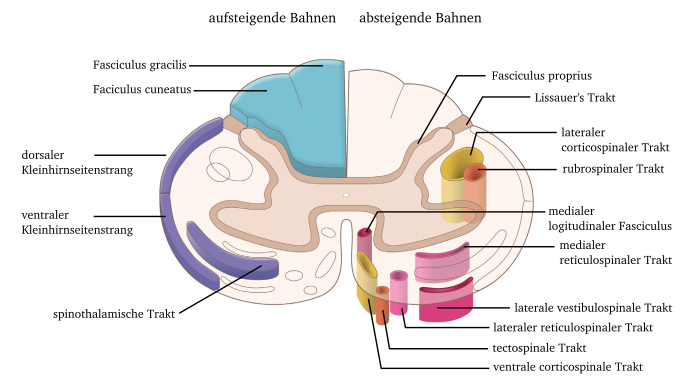
\includegraphics [width = \textwidth]
    {pictures/somatosensory/aufabsteigendeBahnen_Rueckenmark.png}
    \caption[Auf- und Absteigende Bahnen im Rückenmark]{\textbf{Auf- und Absteigende Bahnen im Rückenmark}\\ Zur besseren Veranschaulichung der Bahnen sind die Bahnen in der Abbildung nach absteigenden Bahnen auf der linken Seite und absteigenden Bahnen auf der rechten Seite aufgeteilt. Beide Gruppen kommen jeweils gespiegelt auch auf der anderen Seite vor.
    \textsuperscript{\cite[8]{crossman2014neuroanatomy}}}
    \label{fig:bahnen_rueckenmark}
\end{figure}

\subsubsection*{Nucleus gracilis und Nucleus cuneatus - Medulla}

Die Axone des \textit{Fasciculus~gracilis} terminieren im \textit{Nucleus~gracilis} in der Medulla. Auf gleicher Ebene der Medulla enden auch die Axone des \textit{Fasciculus~cuneatus} im \textit{Nucleus~cuneatus}. Zusammen werden die beiden Kerne auch Hinterstrangkerne oder im englischen dorsal column nuclei genannt. in Abbildung~\ref{fig:nucleus_cuneatus} kann man den Nucleus~cuneatus (gelb) sehen. Der Nucleus liegt dorsal des Kerngebiets des Trigeminusnervs (Sp5I) und lateral des vierten Ventrikels (4V). Die Abbildung zeigt nicht den Nucleus gracilis.
\\
\noindent
Beide Nuclei sind zylindrisch geformt und in rostrocaudaler Richtung ausgedehnt. Die afferenten Neuronen aus einer Hautregion enden in der rostrocaudalen Ausdehnung auf einer Linie und verschiedene Hautregionen werden lateral-medial repräsentiert. Die somatosensorische Repräsentation auf dieser Ebene gleicht einem auf dem Rücken liegenden, kopflosen Homunculus. Dabei liegen die distalen Körperregionen lateral und die proximalen Hautregionen medial in den Nuclei. Die taktilen und propriozeptiven Informationen des Kopfes (Kap.~\ref{sec:somatokopf}) werden in angrenzenden \textit{Nucleus principalis nervi trigemini} repräsentiert \textsuperscript{\cite[22]{kandel2013principles}}. 
\\
\begin{figure}[H]
    \centering
    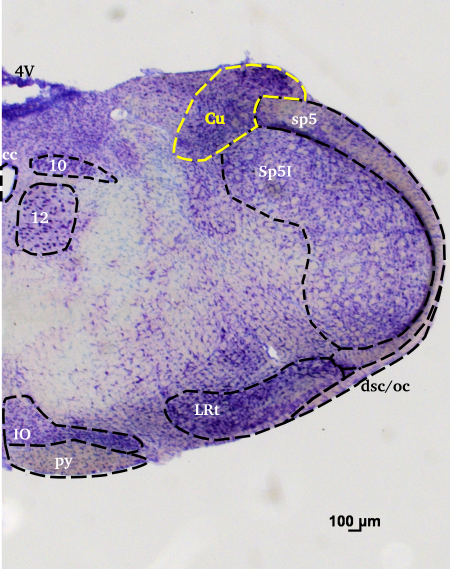
\includegraphics{pictures/somatosensory/nucleus_cuneatus.png}
    \caption[Lage des \textit{Nucleus cuneatus} in der Medulla]{\textbf{Lage des \textit{Nucleus cuneatus} in der Medulla}\\
    Nissel-Färbung der Rattenhirns auf der Höhe der Medulla (N02\_3R). Der Ausschnitt zeigt die rechte Seite vom Zentralkanal (cc) bis zum Trigeminusnerv (sp5). Oberhalb des Kerngebiets des Trigeminusnervs (SP5I) liegt der Nucleus~cuneatus (Cu). Die Schnittebene beinhaltet sowohl Teile der Medulla, daran zu erkennen, dass der vierter Ventrikel (4V) angeschnitten ist, als auch Teile des Rückenmarks, daran zu erkennen, dass der Zentralkanal (cc) zu sehen ist. Weitere Kerngebiete sind: der dorsaler Kern des Nervus vagus(10), Kern des Nervus hypoglossus (12), die untere Olive (IO) und der Nucleus reticularis lateralis (LRt). Ebenfalls zu sehen sind: die Pyramidenbahn (py), der dorsaler spinocerebellarer Tract/olivocerebraler Tract (dsc/oc) und der Trigeminusnerv (sp5).}
    \label{fig:nucleus_cuneatus}
\end{figure}

\subsubsection*{Der Mediale Lemniscus}
In den Hinterstrangkernen ist die erste synaptische Verbindung im lemniskalen System. Von den primär afferenten Axonen aus dem Rückenmark wird das Signal an die Nervenfasern des \textit{medialen~Lemniscus} weiter geleitet. Diese kreuzen die Mittellinie auf der Höhe der Medulla und verlaufen anschließend contralateral \textsuperscript{\cite[22]{kandel2013principles}}. 
Der \textit{mediale~Lemniscus} liegt ventral-medial in der Medulla und zieht von der Medulla bis in den Thalamus im Diencephalon. Die Veränderung der Lage des \textit{medialen~Lemniscus} \index{medialer Lemniscus} kann man in Abbildung \ref{fig:medialer_lemniscus} verfolgen. Er beginnt schon auf der Höhe des Nucleus cuneatus (Abb.~\ref{fig:somato_pathway}) und zieht sich dann ventral-medial unterhalb des Aqueduct (Abb.~\ref{fig:medialer_lemniscus}A) weiter nach rostral. Dabei verändert er seine Lage in sofern, dass er von ventral-medial nach medial-lateral (Abb.~\ref{fig:medialer_lemniscus}B) zieht. Der mediale~Lemniscus zieht sich auf der Höhe des dritten Ventrikels (Abb.~\ref{fig:medialer_lemniscus}C) zentral im Diencephalon bis in den Thalamus.

\begin{figure}[H]
    \centering
    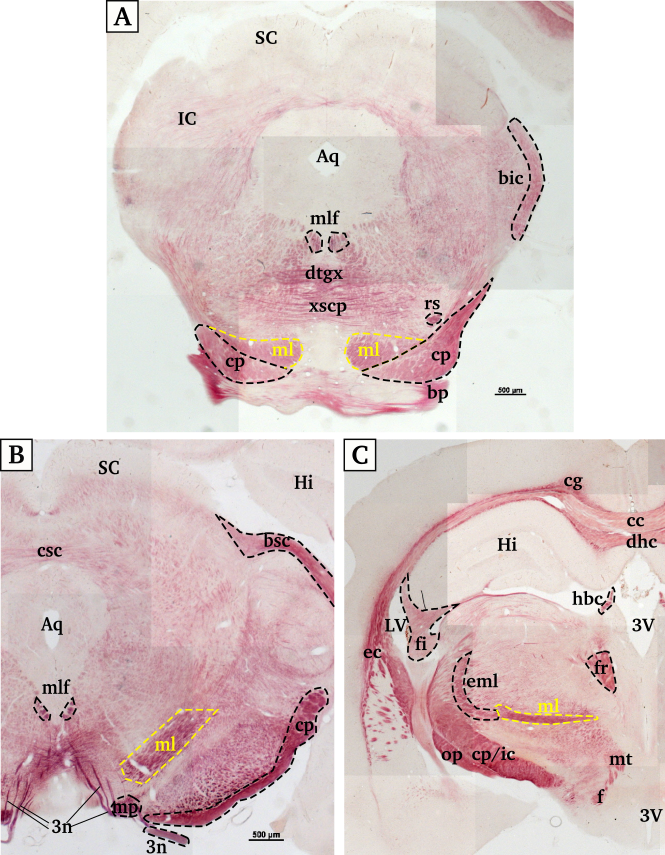
\includegraphics[width = 0.9\textwidth] {pictures/somatosensory/medial_lemniscus.png}
    \caption[Verlauf des \textit{medialen Lemniscus}]{\small{\textbf{Verlauf des \textit{medialen Lemniscus}}\\
    Faserschnitte auf der Höhe des Mesencephalons (A \& B) und des Diencephalons (C). Man kann den Verlauf des medialen Lemniscus in der Schnittserie über 3450~$\mu$m verfolgen.\\
    \textbf{A} (F14\_4P): Colliculus superior (SC), Colliculus inferior (IC), Aqueduct (Aq), Brachium des IC (bic), brachia pontis (bp, eng.: middle cerebellar peduncle), Großhirnstiele (Pedunculi cerebri) (cp), dorsal tegmental decussation (dtgx), Fasciculus longitudinalis medialis (mlf), rubrospinaler tract (rs), decussation des SC peduncels (xscp).
    \textbf{B} (F17\_3P): Nervus oculomotorius (3n), Hippocampus (Hi), Brachium des SC (bsc), Kommissur des SC (csc), mammillary peduncle (mp).
    \textbf{C} (F20\_3P): dritter Ventrikel (3V), lateraler Ventrikel (LV), zentrale Kommissur (cc), cingulum (cg), dorsale Hippocampuskommissur (dhc), Capsula externa (ec), external medullary lamina (eml), Fornix (f), Fimbria (fi), fasciculus retroflexus (fr), Commissura habenularum (hbc), Kapsula interna (ic), mammillothalamic tract (mt), optischer tract (op)}}
    \label{fig:medialer_lemniscus}
\end{figure}

\subsubsection*{Thalamus}
Die Informationen aus den Hautschichten von den Meissner-, Merkel- und Pacini-Rezeptoren, die über den die primär afferenten Neuronen und den \textit{medialen Lemniscus} kommen, werden im lateralen und medialen Nucleus ventralis posterior (eng.: lateral and medial
ventral posterior nuclei) verarbeitet. Proprioceptive Informationen aus den Gelenken und dem Bauchraum werden über den medialen Lemniscus an den oberen Nucleus ventralis posterior (eng.: superior ventral posterior nucleus) weitergeleitet \textsuperscript{\cite[22]{kandel2013principles}}. 
In der Nisselfärbung des Rattenhirns ist keine Abgrenzung der einzelnen Nuclei des Thalamus sichtbar. Der Thalamus als Verschaltungszentrale des Diencephalons liegt bei der Ratte zentral unter dem dritten Ventrikel (3V, Abb.~\ref{fig:thalamus_somato}) und oberhalb des Hypothalamus. 
Am Beispiel des Menschen werden in Kapitel \label{subsubsec:thalamus} die einzelnen Kerne im Thalamus gezeigt, wobei die Lage der somatosensorischen Kerne gut in Abbildung \ref{fig:thalamus_nuclei}~A~\&~B zu sehen ist.
Die zweite synaptische Verschaltung im Thalamus gibt die Informationen an die Neuronen der thalamisch-corticalen Verbindung weiter, welche die Informationen dann an den primären somatosensorischen Cortex leitet.

\begin{figure}[H]
    \centering
    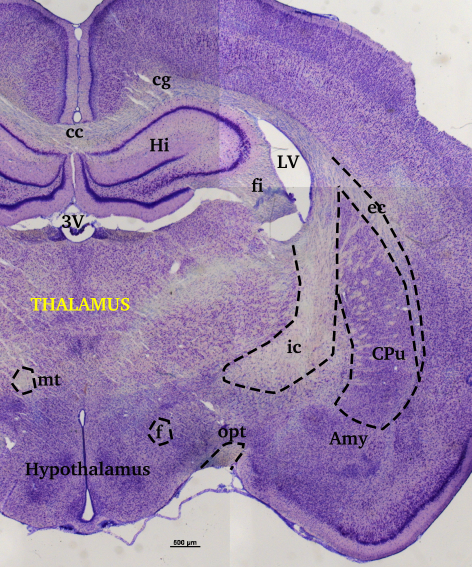
\includegraphics{pictures/somatosensory/thalamus_somato.png}
    \caption[Thalamus]{\textbf{Thalamus}\\
    rechte Gehirnhälfte (N23\_3P) der Ratte auf der Höhe des Thalamus und des dritten Ventrikels (3V). Auf der selben Höhe in Schnitt sind als prominente Hirnstrukturen der Hippocampus (Hi), der Hypothalamus und die zentrale Kommisur (eng.: corpus callosum, cc) zu sehen. Weitere Strukturen sind: der Cortex, Amygdala (Amy), Caudate Putamen (CPu), Cingulum (cg), äußere Kapsel (ec), Fornix (f), Fimbria (fi), innere Kapsel (ic), laterale Ventrikel (LV), mammillothalamic tract (mt), optische Bahn (opt)}
    \label{fig:thalamus_somato}
\end{figure}

\subsubsection*{Primärer Somatosensorischer Cortex}
\label{subsubsec:S1}
Der somatosensorische Cortex liegt beim Menschen auf dem postzentralen Gyrus, direkt hinter dem \textit{Sulcus centralis}. Der primäre somatosensorische Cortex (S1) setzt sich aus den Brodmann-Arealen 3a, 3b, 1 und 2 zusammen und endet anterior im Sulcus centralis und grenzt dort an den primären Motorcortex (Brodmann-Areal 4). Posterior des S1 liegt der posterior Parietalcortex mit den Brodmann-Arealen 5 und 7. In Abbildung \ref{fig:S1_Cortex} ist ein horizontal Schnitt durch die verschiedenen Areale des primären somatosensorischen Cortex und den angrenzenden Strukturen zu sehen \textsuperscript{\cite[23]{kandel2013principles}}. 

\begin{figure}[H]
    \centering
    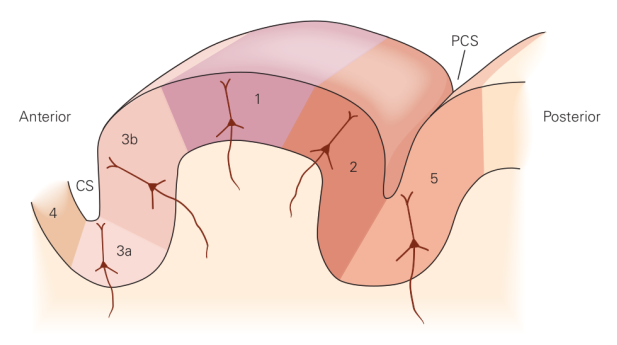
\includegraphics{pictures/somatosensory/S1_Cortex.png}
    \caption[Primärer Somatosensorischer Cortex]{\textbf{Primärer Somatosensorischer Cortex (S1)}\\
    Der primäre somatosensorische Cortex (S1) setzt sich aus den Brodmann-Arealen 3a, 3b, 1 und 2 zusammen und endet anterior im Sulcus centralis (CS) und grenzt dort an den primären Motorcortex (Brodmann-Areal 4). Posterior des S1 liegt der posterior Parietalcortex mit den Brodmann-Arealen 5 und 7 er grenzt sich vom postzentralen Gyrus durch den postzentralen Sulcus (PCS) ab.
    \textsuperscript{\cite[23]{kandel2013principles}}}
    \label{fig:S1_Cortex}
\end{figure}

Betrachtet man den somatosensorischen Cortex in seiner Ausdehnung entlang des Sulcus centralis, wie auch die Schnittebene in Abbildung~\ref{fig:somato_pathway} verläuft, wird nochmal die Somatotopie deutlich. Hierbei ist vor allem der Unterschied zwischen den Tieren sehr prominent. Die somatosensorischen Informationen auf der Hautoberfläche unterscheiden sich in ihrer Größe der rezeptiven Felder und in ihrer daraus resultierenden Relevanz. Auf Grund dessen werden einige Körperregionen mehr repräsentiert als andere eine Darstellung dieser Überrepräsenation ist der Homunculus (Abb.~\ref{fig:somato_homunculus}). Der Homunculus der Ratte ähnelt der des Hasens. 
\\

\begin{figure}[H]
    \centering
    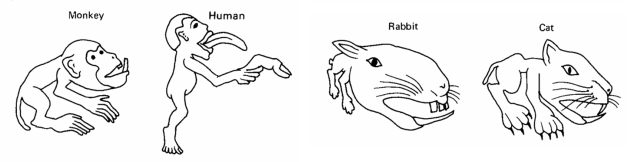
\includegraphics[width = \textwidth] {pictures/somatosensory/homunculus.png}
    \caption[Homunculus]{\textbf{Homunculus}\\
    Homunculi vom Affe (oben links), Menschen (oben rechts), Hase (unten links) und von der Katze (unten rechts).}
    \label{fig:somato_homunculus}
\end{figure}

\newpage
Areal~3b bekommt die Informationen aus den bewussten Mechanorezeptoren der Haut. In diesem Cortexareal werden vor allem die Wahrnehmung der taktilen Reize und deren Form und Textur verarbeitet, wogegen in Areal~3a die Wahrnehmung aus der Körperhaltung und der Proprioception verarbeitet wird. Areal~1 und 2 erhalten ihre Informationen aus Areal~3b. In Areal~1 werden die Informationen aus der strukturellen Beschaffenheit des Objekts weiterverarbeitet und in Areal~2 diese über die Größe und Gestalt. Alle vier Areale des primären somatosensorischen Cortex projizieren in den sekundären somatosensorischen Cortex (S2) \textsuperscript{\cite[12]{neurowissenschaften_baer}}.
\\
\noindent Der sekundäre somatosensorische Cortex liegt unterhalb des primären somatosensorischen Cortex und ist für die Verarbeitung der Informationen aus beiden S1 zuständig. Über den Corpus callosum erhält er die Informationen aus der jeweils anderen Hirnhälfte. Er verarbeitet die bilateralen rezeptiven Felder und ist für den Lerntransfer zwischen den Seiten zuständig. Der S2 ist auch für die generelle Aufmerksamkeit bezüglich taktiler Informationen zuständig \textsuperscript{\cite[12]{neurowissenschaften_baer}}.

Im Gegensatz zu der Lage des somatosensorischen Cortex beim Menschen, steht die Lage bei der Ratte. Da Ratten ein lisencephales Gehirn besitzen und bei diesen Tieren auch kein Sulcus centralis ausgebildet ist, ist die Lokalisation des Areals nicht anhand dessen zu bestimmen. Anhand der Schichtung und Färbungen wurde der somatosensorische Cortex bei der Ratte identifiziert (Abb.~\ref{fig:S1_Cortex_Ratte}). Die Neuronen in dem Teil des Cortex (anterior parietal region) wurden durch eine stark ausgeprägte granuläre Schicht IV und der stärksten Myelinisierung aller Cortexareale identifiziert. \textsuperscript{\cite[22]{paxinos2014rat}}
\\
\begin{figure}[H]
    \centering
    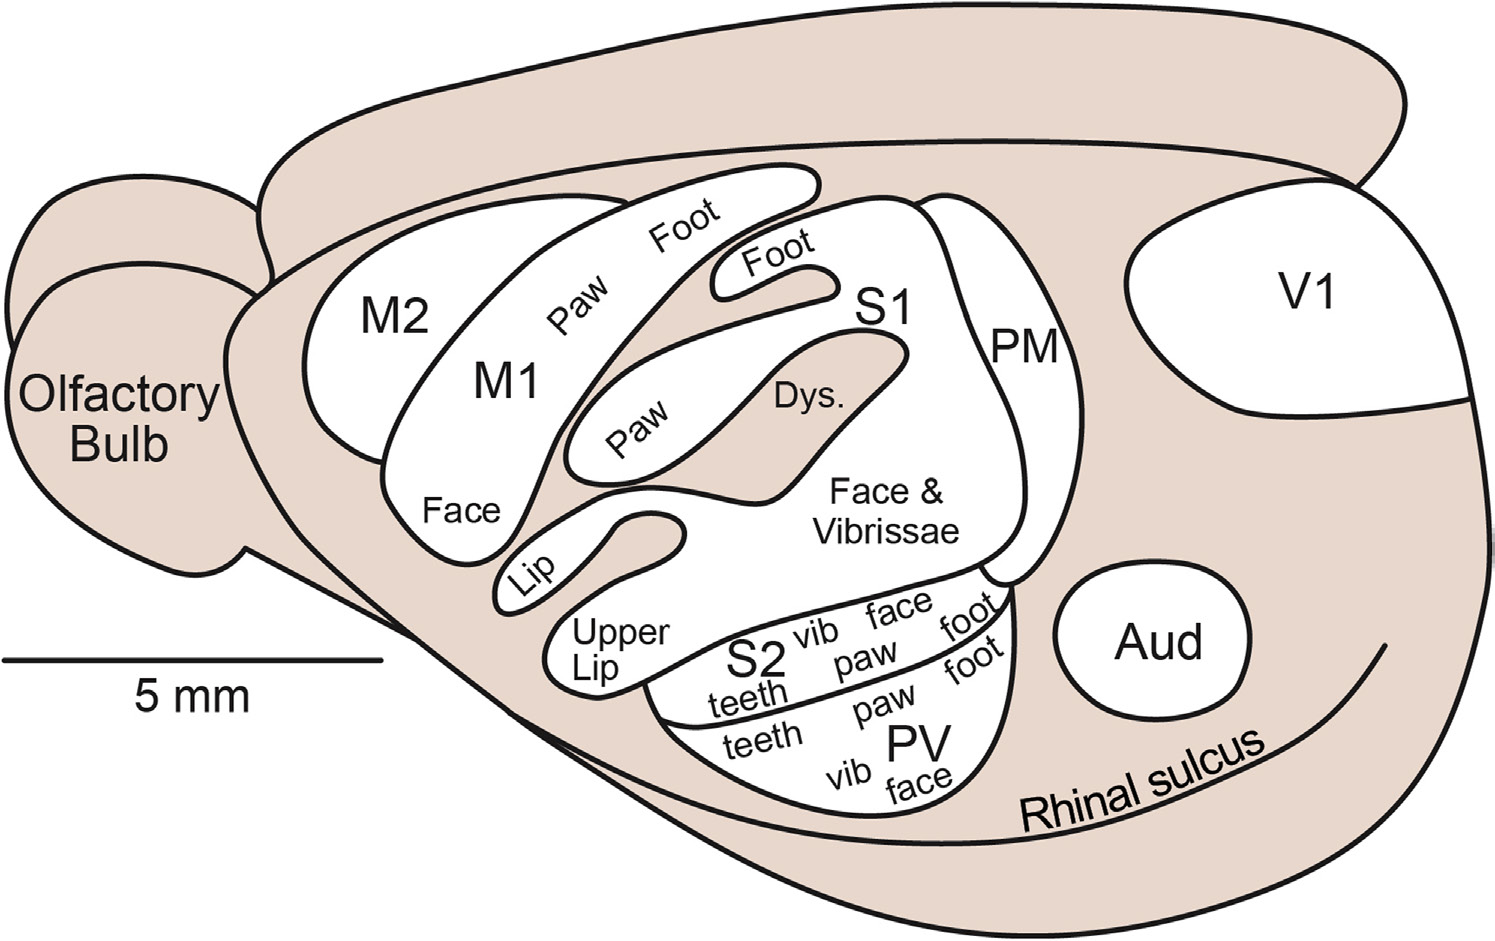
\includegraphics[width = 0.8\textwidth] {pictures/somatosensory/Somato_cortex_ratte.png}
    \caption[Somatosensorischer Cortex der Ratte]{\textbf{Somatosensorischer Cortex der Ratte}\\
    primärer (S1) und sekundärer (S2) somatosensorischer Cortex mit der Repräsentation der einzelnen Körperregionen. Außerdem ist die \textit{Fissura rhinalis} (rhinal sulcus) gezeigt welche den Neocortex vom Archicortex trennt. Anterior vom somatosensorischen Cortex ist der Motorcortex mit primären (M1) und sekundärem (M2) Motorcortex. Ventral des S2 liegt das parietal ventral somatosensorische Areal (PV) und posterior das posteriore mediale Areal (PM). Als Reverenz sind noch der Auditorische Cortex (Aud) und der Visuelle Cortex (V1) gezeigt. \textsuperscript{\cite[24]{paxinos2014rat}}}
    \label{fig:S1_Cortex_Ratte}
\end{figure}

\subsubsection*{Somatosensorische Bahnen}

\begin{figure}[H]
    \centering
    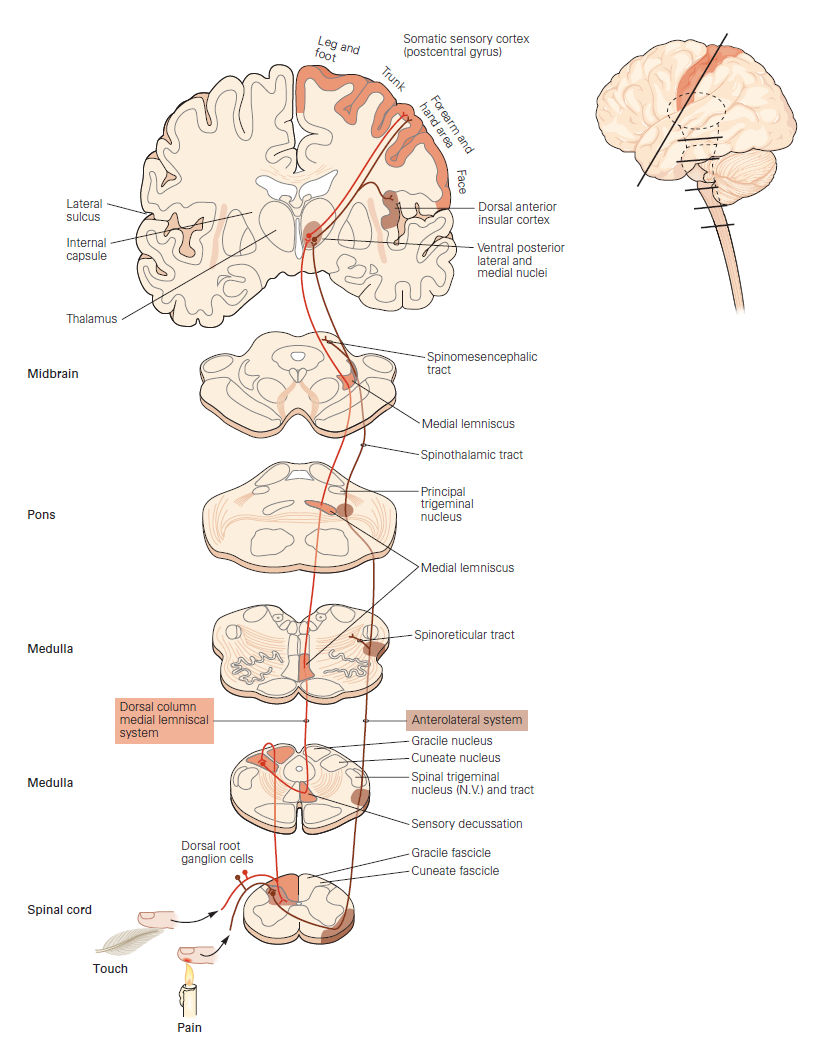
\includegraphics{pictures/somatosensory/pathway_somatosensory2.png}
    \caption[Aufsteigende Bahnen der Somatosensorik]{\textbf{Aufsteigende Bahnen der Somatosensorik}\\
    Die aufsteigenden Bahnen der Somatosensorik sind getrennt in das lemniskale (rot) und das anterolaterale (braun) System. Beginnend im Rückenmark bis zu zum primären somatosensorischen Cortex posterior vom \textit{Sulcus centralis}. Die Bahnen sind am Beispiel des Menschen schematisch dargestellt und sind auf den Ebenen des Rückenmarks, der Medulla, der Pons, des Mittelhirns und des Cortex zu verfolgen.
    \textsuperscript{\cite[22]{kandel2013principles}}}
    \label{fig:somato_pathway}
\end{figure}

\newpage    
\subsubsection{Schmerz und Temperatursinn (anterolaterales System)}
Der Schmerz- und Temperatursinn hat vor allem eine schützende Funktion auf unseren Körper. Er warnt uns vor Verletzungen oder zu großer Hitze, worauf wir dann reflexartig reagieren und zurückweichen oder die Verletzung behandeln. Der Schmerz \textcolor{red}{entspringt} von den somatosensorischen Strukturen in der Haut und wird von dort zu den höheren Gehirnarealen weitergeleitet. 

\subsubsection*{Rückenmark}

Die meisten der Nozizeptoren sind einfache Nervenendigungen primärer sensorischer Faser und können generell in drei Gruppen eingeteilt werden, die thermischen, mechanischen und polymodalen Nozizeptoren \textsuperscript{\cite[24]{kandel2013principles}}. Auch die Zellkörper der Nozizeptoren des Körpers liegen im dorsalen Wurzelganglion und terminieren im Hinterhorn des jeweiligen Segments. Ihre Synapsen konzentrieren sich in den Schichten I, IV, V, VII, und X des Hinterhorns (Abb.~\ref{fig:graymatter}) \textsuperscript{\cite[25]{paxinos2014rat}}.
\\
\\

\begin{figure}[H]
        \centering
        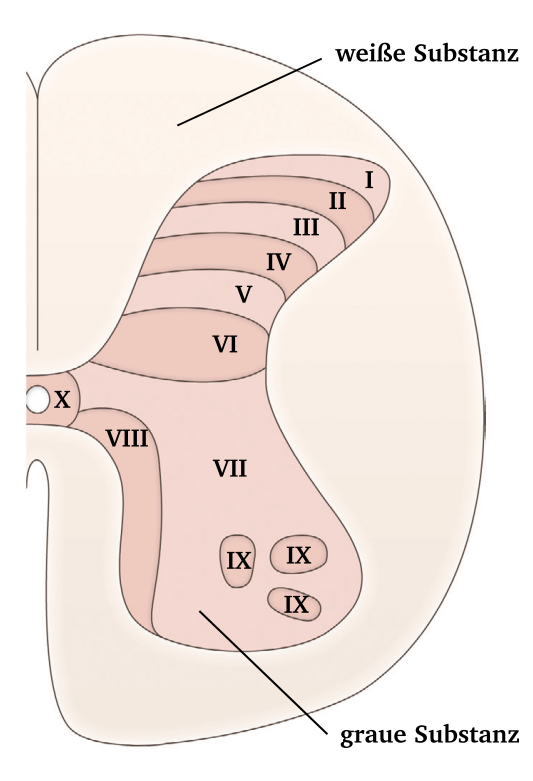
\includegraphics[width = 0.5\textwidth]
        {pictures/somatosensory/gray_matter.png}
        \caption[Schichten in der grauen Substanz des Rückenmarks]{\textbf{Schichten in der grauen Substanz des Rückenmarks} Die Abbildung zeigt schematisch die rechte Seite des Rückenmarks mit weißer und grauer Substanz. Die Schichten der grauen Substanz beginnen im Hinterhorn mit Schicht I und gehen bis Schicht VIII im Vorderhirn. Die Schicht XI liegt in Schicht VIII und Schicht X umgibt den Zentralkanal.
        \cite[8]{crossman2014neuroanatomy}}
        \label{fig:graymatter}
    \end{figure}

\newpage
Diese synaptische Verbindung verbindet die Nozizeptoren mit den spinothalamischen Neuronen. Wie der Name dieser Neuronen schon sagt ziehen die Neuronen vom Rückenmark bis in den Thalamus. Die Zellkörper der Neurone liegen in der grauen Substanz des Rückenmarks, während die Axone in der weißen Substanz des Rückenmarks parallel zum Verlauf der Wirbelsäule in Bahnen auf- und absteigen. Die Axone der spinothalamischen Zellen kreuzen auf der Ebene der ersten Synapse die Mittellinie und steigen in der contralateralen weißen Substanz zum lateralen Bereich des Thalamus auf \textsuperscript{\cite[25]{paxinos2014rat}}. Bei Ratten bildet die größte Gruppe der spinothalamischen Neurone, die welche auf der Höhe der Halswirbelsäule der grauen Substanz entspringen.


\subsubsection*{Thalamus}
Die aufsteigende spinothalamische Bahn im Rückenmark ist anhand ihrer Verbindung von Rückenmark und Thalamus benannt und verläuft ventral des Vorderhorns (Abb.~\ref{fig:bahnen_rueckenmark}). Auch diese Neurone sind somatotopisch organisiert. Die Axone aus Schicht I steigt im laateralen Funiculus, wohingegen die Axone aus den Schichten IV, V und X in der ventralen weißen Substanz aufsteigen und in den medialen und intralaminaren Thalamus projizieren \textsuperscript{\cite[25]{paxinos2014rat}}. 
Mehrere Nuclei des Thalamus verarbeiten die Informationen aus dem anterolateralen Sytem. Die wichtigsten zwei Gebiete sind die lateralen und der medialen Kerngebiete. 
Die lateralen Kerngebiete bestehen aus dem ventro-posterior medialen Nucleus, dem ventro-posterior lateralen Nucleus und dem posterioren Nucleus. Sie erhalten Informationen über nociception-spezifische Neurone und von Neuronen mit einem breiten dynamischen Spektrum. Dieses Kerngebiet beschäftigt sich deshalb unter anderem mit der präzisen Lokalisation einer Verletzung und der Übertragung der Informationen als bewussten Schmerz\textsuperscript{\cite[24]{kandel2013principles}}.
\\
\noindent Die medialen Kerngebiete des Thalamus setzen sich aus dem zentral-lateralen Nucleus und dem intralaminaren Komplex zusammen. Sie bekommen unter anderem Input aus dem spinothalamischen Tract, aber auch aus der \textit{Formatio reticularis}. Neurone im medialen Thalamus reagieren auf schädigende Stimuli und projizieren in die Basalganglia und den Cortex \textsuperscript{\cite[24]{kandel2013principles}}.

\subsubsection*{Cortex}
Bei Ratten wurde Reaktionen auf einen schädigenden Stimulus im primären somatosensorischen Cortex aufgenommen. Demnach werden hier zum Teil die Informationen aus dem anterolateralen System verarbeitet. Die Neuronen aus dem nociceptiven System befinden sich in der Schicht V und VI des somatosensorischen Cortex, wohingegen sich die mechanorezeptiven Neurone in Schicht II~-~V befinden. Die rezeptiven Felder des Schmerz- und Temperatursinns im Cortex sind vergleichsweise zu den der mechanosensorischen rezeptiven Felder größer und sie sind meist inhibitorisch \textsuperscript{\cite[25]{paxinos2014rat}}.
\\
\noindent Im Gegensatz dazu steht die Verarbeitung der Schmerz- und  Temperaturwahrnehmung beim Menschen. Einige der Neuronen im \textit{Gyrus cinguli}, oberhalb des \textit{Corpus callosum}, und der Inselrinde (\textit{Cortex insularis}), innerhalb des Sulcus lateralis, reagieren sark und ausschließlich auf Reize aus dem nociceptiven somatosensorischen System. Der Gyrus cinguli ist wie schon in Kapitel \textcolor{red}{Auf deas Kapitel Faltung der Großhirnrinde verweisen} beschrieben, ein Teil des limbischen Systems. Es wird vermutet, dass das limbische System bei der Verarbeitung von Gefühlszuständen assoziiert mit der Schmerzwahrmnehmung beteiligt ist. Neuronen des Thalamus projizieren direkt zur Inselrinde, vor allem aus dem medialen und venteroposterior-medilen Nucleus des Thalamus. Die Inselrinde verarbeitet hauptsächlich Informationen über den Zustand innerhalb des Körpers und wirkt bei der autonomen Reaktion des Körpers auf den Schmerz mit \textsuperscript{\cite[24]{kandel2013principles}}.

\subsubsection*{Spinomesencephalischer Tract und  Spinoreticularer Tract}

Sowohl der Spinomesencephalische Tract als auch der Spinoreticuläre Tract sind Abzweigungen vom spinothalamischen Tract. Es ist bekannt, dass der spinoreticuläre Tract bei der absteigenden Schmerzunempfindlichkeit und bei autonomen Regulationen eine Rolle spielt. Der Spinomesencephalische Tract ist an der Schmerzwahrnehmung beteiligt, wobei er für den motivational-affectiven Aspekt, also für die Vermeidung von Schmerz weil er unangenehm ist, zuständig ist. Aus diesem Grund ist der Spinomesencephalische Tract auch beim auslösen von Aktivität im absteigenden Kontrollsystem involviert \textsuperscript{\cite[24]{kandel2013principles}}.


\newpage
\subsection{Somatosensorik des Kopfes (trigeminales System)\index{System! trigeminales}}
\label{sec:somatokopf}
Die Somatosensorik des Kopfes beinhaltet beim Menschen die Informationen aus den somatosensorischen Rezeptoren von Gesicht und Mund. Bei einigen Säugetieren kommen noch wichtige Informationen aus den Vibrissen im Gesichtbereich, die sogenannte Viszerosensorik\index{Viszerosensorik}. Die Verarbeitung dieser Informationen über das trigeminale System wird im Folgenden beschrieben und auf die Rolle der Vibrissen wird genauer eingegangen.

\subsubsection*{Vibrissen}
Die Aufgabe von Vibrissen\index{Vibrissa} ist die Nahorientierung und -erkundung, weshalb sie an verhaltensrelevanten Körperteilen vorkommen. Die meisten Säuger, die ihre Nahrung mit der Schnauze ergreifen und nicht mit den Händen, besitzen Vibrissen im Kopfbereich um die Schnauze, aber auch an anderen Körperstellen, wie z.B. unterm Kinn (Wüstenspringmäuse) oder zwischen den Zehen (Katzen), gibt es die Tasthaare. Die Vibrissen sind lange, steige Tasthaare, welche von einem Blutsinus umgeben sind. Die Schnurrbarthaare \index{Schnurrbarthaare|see{Vibrissa}}sind spezialisierte Vibrissen die zusätzlich noch bewegt werden können. 
Die Auslenkung der Vibrissen führt zu einer Aktivierung der freien Nervenendigungen, die im Haarschaft zwischen Haar und Blutsinus liegen \textsuperscript{\cite[5]{heldmaier2003tierphysiologie}}.

\subsubsection*{Nucleus des Trigeminus}
Die freien Nervenendigungen der Vibrissen und die Mechanorezeptoren im Gesicht und Mund bilden zusammen den fünften Hirnnerv (\textit{Nervus trigeminus})\index{CN~V}\index{Nervus trigeminus}. Die Ganglien der Nerven liegen alle außerhalb des Hirnstamm im \textit{Ganglion Gasseri} (eng.: trigeminal ganglion)\index{Ganglion Gasseri}\index{trigeminal ganglion}, wobei eine Großzahl der Neuronen die Vibrissen repräsentiert.
\\
\noindent
Der Trigeminus ist der fünfte Hirnnerv (CN~V)\index{CN V}. je nach Lage in den Schnitten durch das Gehirn ist die Bezeichnung des Trigeminuns unterschiedlich. Auf der Höhe der Medulla ist es noch der spinale Tract des Trigeminus (sp5, Abb.~\ref{fig:somato_Pr5}), wohin gegen auf der Höhe des Aqueducts im Mesencephalon sensorischen Trigeminius (s5, Abb.~\ref{fig:somato_Pr5}) geredet wird. Der Trigeminus ist auch in sich geordnet, wobei die Neurone aus dem Tastsinn vorne im Trigeminuns representiert sind und die neurone aus dem Schmerzsinn hinten.
\\
\noindent
Die Axone des Ganglion Gasseri ziehen auf der Höhe der Pons in den Hirnstamm und teilen sich dort um in den Nucleus principalis des Trigeminus (Pr5, \textit{Nucleus principalis nervi trigemini}) \index{Pr5 !Nucleus principalis} und drei Gebiete, oralis (Sp5O), interpolaris (Sp5I), und caudalis (Sp5C), des spinalen Nucleus des Trigeminus (Sp5, \textit{Nucleus spinalis nervi trigemini}) \index{Sp5 !spinalen Nucleus des Trigeminus}zu ziehen. Alle Gebiete gehören zum \textit{Nucleus trigemini} welcher sich über das Mesencephalon, die Pons und die Medulla zieht\textsuperscript{\cite[5]{heldmaier2003tierphysiologie}}. 
Hinzu kommen Informationen aus dem Nervus facialis (CN~VII), dem Nervus glossopharyngeus (CN~IX) und dem Nervus vagus (CN~X), welche die Hautbereiche um die Ohren, sowie die Nasen und Rachenregion abdecken
\textsuperscript{\cite[12]{neurowissenschaften_baer}}.
\\
\noindent Die Neurone des Nucleus principalis reagieren auf Reize aus dem Kopfbereich, von der Zunge und des Gesichts. Zusammen mit dem Nucleus gracilis und Nucleus cuneatus repräsentieren die drei Nuclei den sensorischen Input des gesamten Körpers. Die Neurone im Nucleus principalis (Pr5, Abb.~\ref{fig:somato_Pr5}) und in Teilen auch die des Nucleus spinalis (Sp5, Abb.~\ref{fig:somato_Pr5}) bekommen die Information aus spezifischen Körperregionen und sind durch Neuropil in Cluster geteilt. Vor allem sind die Cluster die aus den einzelnen Vibrissa gebildet werden in der richtigen Schnittebene gut zu sehen und sind, nach dem Zusammenhang mit den 'Barrels' im Cortex, im Nucleus principalis 'barrelettes' genannt \textsuperscript{\cite[5]{heldmaier2003tierphysiologie}}.

\begin{figure}[H]
    \centering
    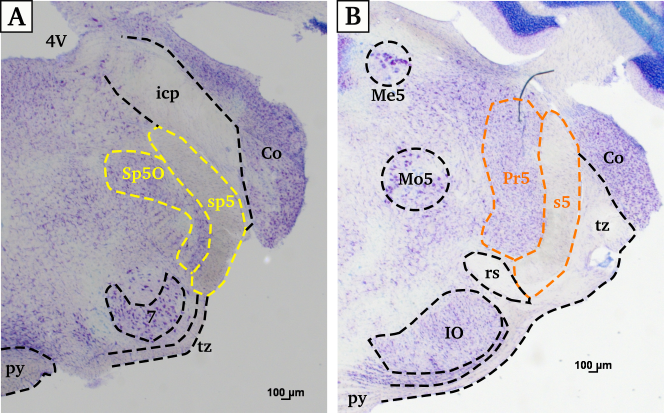
\includegraphics[width = \textwidth]
    {pictures/somatosensory/somato_kopf.png}
    \caption[Nucleus spinalis und Nucleus principalis des Trigeminus]{\textbf{Nucleus spinalis und Nucleus principalis des Trigeminus}\\
     \textbf{A} (N06\_4R): Der Nucleus spinalis oralis (Sp5O) liegt in der Medulla lateral auf der Höhe des Nucleus cochlearis (Co) und doral des Nucleus facialis (7). Des weiteren sieht man den spinalen Trigeminus (sp5) lateral des Nucleus. Weiter Strukturen sind: vierter Ventrikel (4V), inferior cerebelles Peduncle (icp), Pyramidenbahn (py), Trapezkörper (tz)
     \textbf{B} (N09\_3R): Der Nucleus principalis (Pr5) des Trigeminus liegt im Mesencephalon lateral-dorsal auf der Höhe der Inferioren Olive (IO). Die Axone zum Nucleus liegen im Trigeminus (s5). Weitere Strukturen sind: Nucleus cochlearis (Co), Nucleus mesencephalicus des Trigeminus (Me5), Nucleus motorius des Trigeminus (Mo5),  Pyramidenbahn (py), rubrospinaler Tract (rs), Trapezkörper (tz)}
    \label{fig:somato_Pr5}
\end{figure}

\subsubsection*{Nucleus mesencephalicus des Trigeminus}
Einige der Neurone die für die somatosensorische Reizweiterleitung aus dem Kopfbereich zuständig sind, haben ihre Zellkörper nicht im Ganglion Gasseri. Dazu gehören die Neurone die aus den Muskelspindeln kommen, und einige Neurone aus den Vibrissen und Neurone von den Zahnwurzeln. Die Zellkörper diese Neurone sind im Nucleus mesencephalicus des Trigeminus (Me5, Abb.~\ref{fig:somato_Pr5}) \index{Me5 !Nucleus mesencephalicus des Trigeminus}lokalisiert. Die Axone der Neuronen projizieren in den dorsomedialen Bereich des Nucleus principalis \index{Pr5 !Nucleus principalis} \textsuperscript{\cite[5]{heldmaier2003tierphysiologie}}.

\subsubsection*{Thalamus und Cortex}
Die Axone aus dem Nucleus principalis kreuzen die Mittellinie und stoßen zum medialen Lemniscus hinzu und ziehen in den Thalamus. Die Axone aus dem trigeminalen System ziehen in den medialen Part des Thalamus. Im Thalamus wird über synaptische Verschaltung die Information an die Nervenzellen der thalamocorticalen Verbindung zum primären somatosensorischen Cortex (S1) weiter gegeben. 
Wie schon in Kapitel \ref{subsubsec:S1} beschrieben ist S1 für die Verarbeitung der somatosensorischen Reize aus dem Körper verantwortlich. Bei Ratten kommt die meisten somatosensorischen Informationen aus den Vibrissen. Von jeder Vibrisse gehen um die 100 myelinisierte Nervenfasern ab. Über den Trigeminus werden die Informationen erst in den Nucleus principalis geleiten, von dort ziehen andere Neurone weiter in den Thalamus und von dort in den Cortex. Die Neuronen enden im Cortex in abgegrenzten Strukturen, sogenannten 'Barrel' (Abb.~\ref{fig:barrelcortex}B). Die Anzahl der 'Barrels' entsprechen den der Vibrissen und die 'Barrels' sind nach ihrem Aufbau benannt. In der Nissel-Färbung in Abbildung~\ref{fig:barrelcortex}C sieht man die Neurone dicht gepackt um weniger dichte Bereiche. Die Wände der Tonnen (eng.: barrels) sind die dicht gepackten Neurone und das Innere die weniger dicht gepackten Bereiche, daher der Name 'Barrels' \textsuperscript{\cite[8]{smith2008biology}}. 

\begin{figure}[H]
    \centering
    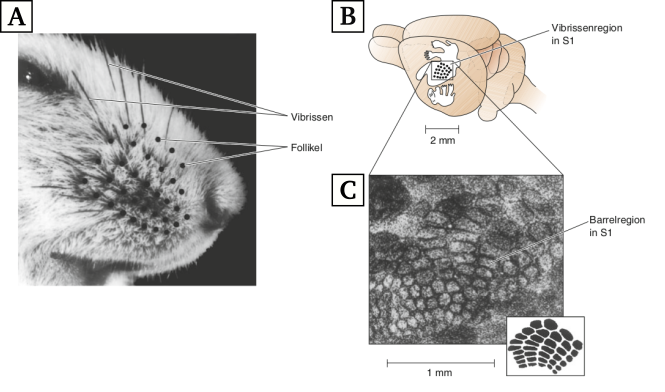
\includegraphics[width = \textwidth] {pictures/somatosensory/barrelcortex.png}
    \caption[Barrelcortex]{\textbf{Barrelcortex}\\
    \textbf{A}: Die Lage der Vibrissen am Beispiel einer Maus \textbf{B}: schematische Darstellung des primären somatosensorischen Cortex (S1) mit der Lage der 'Barrel' (englisch für Tonne, nach dem Aussehen der einzelnen cortikalen Areale jeder Vibrisse) in S1. Die 'Barrel' sind analog zur Lage der Vibrissen zueinander angeordnet. \textbf{C}: Barrelregion innerhalb von S1. Der Schnitt durch die 'Barrel' ist horizontal zum Cortex angelegt und mit Hilfe einer Nissel-Färbung angefärbt. Die Abbildung unten rechts, zeigt nochmal die Anordnung der Barrel in fünf Reihen wie auch in \textbf{A} zusehen ist.
    \textsuperscript{\cite{barrelcortex2008}}}
    \label{fig:barrelcortex}
\end{figure}


\newpage
\section{Spezielle sensorische Bahnen}
% verweis auf dieses Kapitel mit \ref{sec:spezsens}
\label{sec:spezsens}
Die speziellen sensorischen Bahnen umfassen unter anderem die Hörbahn, die Sehbahn und die Riechbahn, womit sich in diesem Kapitel vor allem beschäftigen wird. Diese drei speziellen sensorischen Bahnen spielen sowohl bei der Ratte als auch beim Schaf die zentrale Rolle. Es gibt weiter spezialisierte Sinne wie zum Beispiel den elektrischen Sinn bei Fischen, die beiden chemischen Sinne für Geruch und Geschmack und der Magnetsinn bei Zugvögeln \textsuperscript{\cite{smith2008biology}}. Diese werden nicht in dieser Zusammenfassung behandelt, spielen aber bei anderen Tierarten eine tragende Rolle und sollten aus diesem Grund hier kurz erwähnt werden.

\subsection{Hörbahn}

Das auditorische System ist für die Verarbeitung von Schallwellen, die über die Luft oder Wasser übertragen und vom System empfangen werden, zuständig. Vibrationen die über den Untergrund oder festes Substrat übertragen werden und mechanisch wahrgenommen werden, gehören zum Vibrationssinn der eng verwandt mit dem auditorischen Sinn ist.
\\
\noindent Dabei hat der auditorische Sinn zwei Aufgaben: zum einen die Detektion des Schalls und die Lokalisation der Schallwelle. Das Richtungshören ist nicht für alle Tiere möglich und ist auch bei den Tieren die dazu befähigt sind, nicht im gesamten Hörbereich gleich genau \textsuperscript{\cite[18]{penzlin2005tierphys}}.

\subsubsection*{Spiralganglion}
Die Funktion unserer Ohren ist die Energie eines akustischen Signals von der Außenwelt einzufangen und von einem mechanischen Signal in ein elektrisches Signal umzuwandeln. Diese Umwandlung findet an den inneren Haarsinneszellen in der Cochlea statt. Dort wird durch die Auslenkung der Haarbündel an den inneren Haarsinneszellen (eng.: inner hair cell, IHC) die Zelle depolarisiert oder hyperpolarisiert je nach Auslenkungsrichtung \textsuperscript{\cite[30]{kandel2013principles}}. 
\textcolor{red}{Verbindung von IHC to spiral ganglion cell
dann auf Type 1 und Type 2 fasern eingehen und den unterschied und kurz auf OHC verweisen}
\\
\\
Die Spiralganglien verdanken ihren Namen der spiralförmigen Struktur der Cochlea der sie folgen. Sie formen einen Teil des achten Hirnnerves (CN~VIII), der auch Nervus vestibulocochlearis genannt wird. Ungefähr 30~000 Ganglionzellen im Hörnerv werden durch die inneren Haarzellen innerviert, das macht ungefähr 90\% des Nerves aus. Anhand der Neuronenverteilung in der afferente Bahn wird die funktionale Bedeutung zwischen den inneren und äußeren Haarzellen erkennbar. Dabei wird jedes Axon nur von eine Haarzelle innerviert, aber eine Haarzelle innerviert im Durchschnitt zehn Fasern \textsuperscript{\cite[30]{kandel2013principles}}. 

\begin{figure}
    \centering
    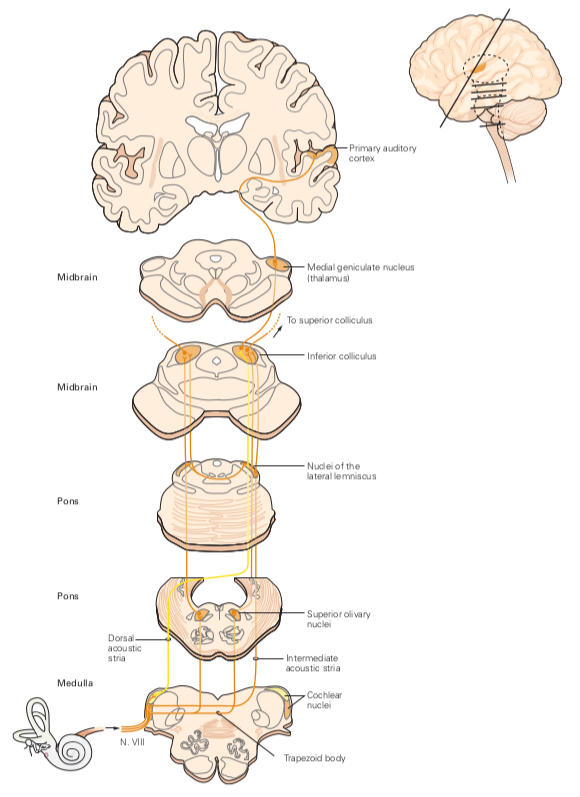
\includegraphics{pictures/auditory/hoerbahn_pathway.png}
    \caption[Hörbahn]{\textbf{Hörbahn}}
    \label{fig:hoerbahn_pathway}
\end{figure}


\begin{itemize}
    \item Funktion of the ear
    \item von einem mechanischen stimulus zu einem chemischen und dann zu einem elektrischen signal
    \item Wie Ableitungen von Haarzellen zeigen, werden sie depolarisiert,
    wenn die Stereocilien in die eine Richtung, und hyperpolarisiert, wenn sie in die andere
    Richtung abgebogen werden (Abb. 11.14a). Wenn eine Schallwelle dazu führt, dass die
    Stereocilien hin- und hergebogen werden, generiert die Haarzelle – ausgehend von einem
    Ruhepotenzial von 70 mV – abwechselnd ein hyperpolarisierendes und ein depolarisie-
    rendes Rezeptorpotenzial
    \item Eine Auslenkung der Stereocilie in die
    eine Richtung erhöht die Spannung am tip-link und damit auch den K plus -Einstrom. Eine
    Auslenkung in die entgegengesetzte Richtung senkt die Spannung am tip-link, sodass sich
    der Kanal vollständig schließen kann und der K plus -Einstrom völlig zum Erliegen kommt.
    Der Einstrom von K plus in die Haarzelle führt zu einer Depolarisation, die wiederum span-
    nungsgesteuerte Calciumkanäle aktiviert (Abb. 11.15b). Das Eindringen von Ca 2plus löst die
    Freisetzung eines Neurotransmitters – wahrscheinlich Glutamat – aus, der die Spiralgan-
    glienfasern aktiviert, die die postsynaptischen Partner der Haarzellen bilden.
    \item Die Haarzellen bilden Synapsen mit Neuronen, deren Zellkörper im Spiralganglion inner-
    halb der Schneckenspindel liegen. Spiralganglienzellen sind bipolare Zellen, ihre Neuriten
    laufen zur Basis und zu den Seiten der Haarzellen, wo sie synaptischen Input erhalten.
    Axone von den Spiralganglien treten in den Hörnerv ein, einen Zweig des Nervus ves-
    tibulocochlearis (VIII. Hirnnerv), der in die Cochleariskerne in der Medulla projiziert\textsuperscript{\cite[11]{neurowissenschaften_baer}}
    \item
    \item The patterns of efferent and afferent connections
    of cochlear hair cells are complementary. Mature inner
    hair cells do not receive efferent input; just beneath
    these cells, however, are extensive axo-axonic synaptic
    contacts between efferent axon terminals and the end-
    ings of afferent nerve fibers. In contrast, efferent nerves
    have extensive connections with outer hair cells on their
    basolateral surfaces. Each outer hair cell receives input
    from several large efferent terminals, which fill the space
    between the cell’s base and the associated Deiters’s cell.
    \item Cochlear Nerve Fibers Encode Stimulus Frequency
    and Intensity
    \end{itemize}

\subsubsection*{Nucleus cochlearis}
   
\begin{itemize}
 \item Nucleus cochleraris: lateral an der Medulla, ipsilaterale Repräsentation
    \item terminierung der inneren haarzellen in cochlear nucleus 
    \item tonotopie 
    \item ipsilaterale monoaurale verschaltung
    \item function des cochlaear nucleus
    \item weiter verschaltung: großteil in die obere olive, ein kleiner teil direkt in den lateralen leminiscus und dessen nuclei 
\end{itemize}


\subsubsection*{Obere Olive}
\begin{itemize}
    \item \textit{Nucleus olivaris superior}
    \item gesamte nuclei der oberen olive für auditorische verarbeitung (welches sind die anderen kerne??)
    \item function: binaurale verschaltung integration von beiden ohren führt zu richtungs hören
    \item laterale obere olive und mntb für Interaurale intensitäts diffrenz
    \item mediale obere olive für interaurale zeit diffrenz ( tielfe töne) warum bei ratten nochmal kleiner???
    \item wo gehen die zellen dann genau hin
\end{itemize}


\subsubsection*{Lateraler Lemniscus}
    \begin{itemize}
        \item nerven aus der oberen olive ziehen durch den nervenstrang der lateraler leminiscus heißt in den inferior colliculus aber manche sind nochmal zwischen geschaltet in den kernen des lateralen leminiscus ( gibts da ihrgend eine regel oder aufteilung welche verschaltet sind und welche nicht??)
        \item was ist dann der grund für die verschaltung und welche funktion hat der laterale leminiscus ????
    \end{itemize}


\subsubsection*{Colliculus inferior}

    \begin{itemize}
        \item 
    \end{itemize}


\newpage
\subsection{Sehbahn}
\begin{itemize}
    \item eye
    \begin{itemize}
        \item kurzer überblick über die entwicklung des auges in der embryonal entwicklung retina aus dem diencephalon
        \item auf grund der evolutionären Entwicklunf ein "inverted" auge wesswegen die retina und die photorezeptoren nach innen weg vom licht gerichtet sind
        \item formung der retina: \cite{smith2008biology} p.287
        \item retinale zellen Stäbchen und zäpfchen und dann bipolar zellen und Ganglienzellen 
        \item vllt was zu den rezeptifen feldern
    \end{itemize}
    \item visual pathway
    \begin{itemize}
        \item 3 verschiedene wege ( vorlesung von oswald IN)
        \item wie heißen die von führen sie hin und wir konzentrieren uns auf einen zentralen und warum
    \end{itemize}
    \item optic nerve von der Retina zum Chiasma opticum
    \item Optic chiasm    \index{Optic chiasm}
    \begin{itemize}
        \item Semidecussation  \index{Decussation!Semi-}
        \item ganglienzellen von der nasalen/medialen seite des auges kreuzen am optic chiasm auf die andere seite des gehirns wärend die laterale seite des auges auf der selben seite weiter projezieren
        ßitem keine verschaltung im optischen chiasma sondern nur eine kreuzung der ganglien zellen
        \item danach optic tract
    \end{itemize}
    \item Optic tract \index{Optic tract}
    \item LGN: nicht gestreift, hinterer Teil das Thalamus \index{Thalamus}, auf Höhe des superior colliculus \index{SC!Superior culliculus}
    \begin{itemize}
        \item lateral am Diencephalon \index{Diencephalon} vorbei
        \item posteriorer part des thalamus
        \item aufbau des LGN unterschied zwischen primaten (6 Schichten) und Ratten bzw. Schafen
        \item kurz was zur funktion der verschaltung auf der ebene ( vllt etwas zu den rezeptive fields aber dann auch schon auf der ebene der retina erwähnen)
        \item von LGN über die optic radiation (welche nicht in den schnitten sichtbar ist) ruaf in den neocortex und in V1 
    \end{itemize}
    \item Magnifikationsfaktor = Dichte der Zellen und wie sie verschaltet sind
    \\
\end{itemize}
\subsection{(Riechbahn)}
\begin{itemize}
    \item vom olfactorischen bulb über den olfactorischen trakt zu einerm der ältesten teile des neocortex zum Pyriformen lappen
    \item weitere neuronen führen dann zum thalamus un die weitern stränge dann in den orbitofrontal lobe \cite{smith2008biology} 
    \item eventuell Dopaminerge Bilder
\end{itemize}

\newpage
\section{Motorische Kerngebiete und Bahnen}
\subsection{Motorische Kerngebiete}
\subsection{Motorische Bahnen zum Hirnstamm}
\subsection{Motorische Bahnen zum Rückenmark}
\begin{itemize}
    \item laterales System: corticospinaler Trakt
    \item laterales System: rubrospinaler Trakt
    \item mediales System: reticulospinaler Trakt (medial,lateral)
    \item mediales System: vestibulospinaler Trakt
\end{itemize}
\subsection{Kleinhirn}
\begin{itemize}
    \item Vestibulocerebellum, Spinocerebellum, Corticocerebellum 
    \item Schichtung
    \item funktionelle Einheiten
    \item Schaltkreise
\end{itemize}
\subsection{(Motorik der Kopfmuskulatur)}
\subsection{(Motorik der Augen)}

\newpage
\section{Integrative Systeme}
\subsection{Limbisches System und Hippocampus}

\subsubsection*{Info zum Hippocampus}

\begin{itemize}

\item \textcolor{blue}{Hallo, ich hatte für meinen Teil was über den Hippocampus gesucht... Aber ich nehme nur die minimale Info rein, aber vielleicht kannst du was davon gebrauchen.. '' oder "" sind wörtliche Zitate. Die Quellen sollten irgendwo in den referneces hier zu finden sein :) LG Jule}

\item "Der Hippocampus (griechisch für„Seepferdchen“) hat für Lernen und Gedächtnis eine große Bedeutung" \cite[Kap.~7]{neurowissenschaften_baer}
	
\item 'The rat HF looks like a C-shaped structure (Fig. 2). Its long axis extends from the septal nuclei of the basal forebrain rostrodorsally, over and behind the diencephalon, into the caudoventral portion of the hemisphere, where HF abuts the rostrally adjacent amygdaloid complex' (Paxinos, Kap.~20)

\item 'Der Hippecampus liegt zum größten Teil im Schläfenlappen an der Medialwand des Seitenventrikeltmterhorns ( >- Abb. 9.16). Mit seinem rostralen Endstück bildet er dort eine tatzenähnliche Struktur (Pes hippocampi, >- Abb. 9.16, 1). Nach hinten oben reicht er, entsprechend der Rotationsbewegung der Hemisphären in der Embryonalentwickltmg, in einem Bogen bis zum kaudalen Ende des Balkens (Corpus callosurn). Von dort aus setzt er sich dann unterhalb des Balkens in die Faserstruktur
des Fomix fort( >- Abb. 9. 16, 4- 6). Der Fomix zieht in
einem Bogen über dem III. Ventrikel nach rostral m1d ventral weiter und endet in den Corpora mammillaria.' (trepel, Kap.~9)

\item Afferenzen:\\
'Afferenzen erhält der Hippocampus besonders zahlreich über den Tractus perforans von der medial des Hippecampus im Gyrus parabippocampalis (auch: Gyrus hippocampi) liegenden Area entorhinalis (auch: Regio entorhinalis). Über diese Region fließen dem Hippocampus u. a. modulierte sensorische lmpulse aus dem Neokortex und dem Rhinencephalon zu. Weiterhin erhält der Hippecampus afferente Fasern aus dem Thalamus, dem Gyrus cinguli, dem Corpus amygdaloideuro und über den Fornix aus dem Septum.' (trepel, Kap.~9)

\item Efferenzen:\\
'Nahezu alle Efferenzen des Hippocampus verlaufen im Fornix. Dieser gibt auf seinem Weg Faserzüge an das Septum, Corpus amygdaloideum sowie den Hypothalamus ab m1d endet mit dem Hauptteil der Fasern in den Corpora maillaria. Hierbei bildet sich der sog. Papez-Neuronenkreis ( >- Abb. 9.17): Der Hippecampus projiziert über den Fornix in die Corpora mammillaria.' (trepel, Kap.~9)

\item FUNKTION: 'Neben der sehr wichtigen Funktion für die Gedächtnisbildung wird der Hippocampus als Bestandteil des limbischen Systems mit endokrinen, vegetativen und emotionalen Vorgängen in Zusammenhang gebracht.' (trepel, Kap.~9)

\item 'der Hippocampus ist für den transfer von Gedächtnisinhalten vom kurzzeit- zum langzeitgedächtnis esentiell' \cite[Kap.~6]{storch2012lehrbuchzoo}

\item gehört zum lymbischen system \cite[Kap.~6]{storch2012lehrbuchzoo}

\item gehört zu den cortikalen arealen/gebieten  \cite[Kap.~6]{storch2012lehrbuchzoo}

\item the hippocampus is involved with aspects of memory storage (Kandel, Kap.1???)

\item 'The hippocampal formation includes the hippocampus, dentate gyrus, and subiculum. The hippocampus and associated cortical regions form the /oor of the temporal horn of the lateral ventricle (Figure 15–12). Together these structures are responsible for the formation of long-term memories about our daily experiences, so-called episodic memories, but are not the permanent storage site of these memories (see Chapter 65).Damage to the hippocampus interferes with people’s ability to form new memories but does not signi0-cantly impair the ability to retrieve old memories.' (Kandel, Kap.~15)

\item 'the hippocampus is thought to store memories temporarily through long-term synaptic plasticity. The hippocampus then transfers these memories to neocortex by inducing a replay in parietal, temporal, and frontal association cortex of activity patterns elicited by recent events.' (Kandel, Kap.~18)

\end{itemize}

\subsection{Basalganglien}

\newpage
\section{generelle Transmittersysteme (monoaminerge Systeme)}
\section{Quantitative Analyse generelle Transmittersysteme (am Beispiel der catecholaminergen Systeme)}
\subsection{Immunohistochemischer Nachweis catecholaminerger Neurone}
Der immunhistochemische Nachweis catecholaminerger Neurone lässt sich in sechs Einzelschritte unterteilen, diese sind in Material und Methoden auf S.xy zu finden.\newline
1. Quenching\newline
Um eine nicht-spezifische Hintergrundsfärbung durch endogene Peroxidasen zu vermeiden, wird im ersten Schritt durch die Zugabe von Wasserstoffperoxidase eine Reaktion unterbunden. \newline
2. Blocken\newline
Vor der Zugabe des ersten Antikörpers müssen zwei Schritte erfolgen: Zum einen sollen die Antikörper ausschließlich an die spezifischen Bindestellen binden, zum anderen muss den Antikörpern der Zugang zu intrazellulären Antigenen ermöglicht werden.
Um nicht-spezifische Protein-Protein-Interaktion zwischen Antikörpern und Proteinen im zu untersuchenden Gewebe zu unterbinden, werden blockende Poteine hinzuegegeben, die kompetetitv and die unspzifische Bindestelle binden. Hierbei binden Fc-Rezeptoren, welche auf Makrophagen und vielen anderen immunologischen Zellen des Gewebe zu finden sind and das Fc-Ende des Antikörpers und führen somit zur unspezifischen Bindung. 
Um die Antigene des zu untersuchenden Gewebes zugänglich zu machen, muss die Zellmembran vorerst mit Detergenzien bahendelt werden, die die Doppellipidschicht durch Verseifung auflockern - die Permabilisierung.\newline
3. Primärer Antikörper\newline
Der primäre Antikörper besitzt eine Fc-Region, die artspezifisch an unsere Host Bindestelle binder und eine Fab-Region, die an das Epitop des Antigens (Tyrosin-Hydroxylase) bindet.\newline
4. Sekundärer Antikörper\newline
Nun bindet die Fc-Region des ersten Antikörpers and die Fab-Region des zweiten Antikörpers. Der zweite Antikörper ist biotyniliert. \newline
5. Der ABC-Complex\newline
Nachdem das Avidin die biotylinielierte Meerrettich-Peroxidase gebunden hat, kann es nun auch an das biotynilierte Ende des sekundären Antikörpers binden. Dieser Schritt dient der Amplifizerung des Signals.\newline
6. DAB Reaktion\newline
Wasserstoffperoxid bindet and die Meerrettich-Peroxidase und oxidiert das DAB, welches reduziert und nun als bräunliches Edukt vorliegt und somit indirekt die erfolgreiche Bindung and das Antigen sichtbar macht.\newline

\subsection{Lage und Größe der Kerngebiete und Projectionsareale}
\subsection{Dopaminerges und Noradrenegres System}
\begin{itemize}
    \item Incertohypothalamic/nigrostriatal System (Dopamin)
    \item Tuberohypophysial System (Dopamin)
    \item Locus coeruleus (Noradrenalin)
\end{itemize}
\subsection{Größenvergleich der Neurone in \textit{substantia nigra} und \textit{locus coeruleus}}



%%%%%%%%%%%%%%%%%%%%%%%%%%%%%%%%%%%%%%%%%%%%%%%%%%%%%%%%%%5%%
% Bibliography

\newpage
\bibliographystyle{unsrt}
\bibliography{references}

%%%%%%%%%%%%%%%%%%%%%%%%%%%%%%%%%%%%%%%%%%%%%%%%%%%%%%%%%%%%%
% Index
\printindex

2n - II optic nerve
3V - 3. Ventrikel\\
3n - III oculomotor nerve\\
4V - 4. Ventrikel\\
5n - V Trigeminus\\
6n - VI nervus abducens\\
\\
Aq - Aquaeductus cerebri\\
Amy - Amygdala\\
ACx - Archicortex\\
\\
CCx - cingulärer Cortex\\
Cu - Nucleus caudatus\\
CPu - Caudoputamen (Striatum)\\
cc - corpus callosum / Balken\\
ChP - choroid plexus\\
Cx - cerebraler Cortex\\
cp - cerebellar peduncle\\
CS - cortical Spine / cortikales Rückenmark\\
Cb - Cerebellum\\
\\
Epi - Epiphyse\\
EO - epithelium olfactorium\\
\\
f - Fornix\\
fi - Fimbria\\
\\
Hi - Hippocampus\\
Hyp - Hypophyse\\
\\
IC - Inferior colliculus\\
ICj - Islands of Calleja\\
\\
LGN - lat. genuculate nuc.\\
lot - lat. olfactory tract\\
LV - lateraler Ventrikel
\\
Med - Medulla\\
MB - mammillary body\\
\\
NCx - Neocortex\\
\\
OB - olfactory bulb / Riechkolben\\
ox - chiasma opticum\\
ot - olfactory tract / olfaktorischer Trakt\\
\\
Pon - Pons\\
PM - Pia mater\\
\\
RF - rhinal fissure\\
\\
SC - Superior colliculus / Colliculus inferior\\
\\
Th - Thalamus\\
Teg - Tegmentum\\
tz - trapezoid body / Trapezkörper\\
TC - Truncus cerebri / Hirnstamm\\
Tu - olfactory tubercle\\
\\
Ve - Velum\\
\\



\end{document}


